\documentclass[conference]{IEEEtran}
\newcommand*{\rootPath}{../}
\usepackage{url}

% math and cs
% \usepackage[]{algorithm2e}
\usepackage[linesnumbered,lined,boxed,commentsnumbered]{algorithm2e}
\usepackage{amsmath}
\usepackage{amssymb}
\usepackage{mathrsfs}
\newtheorem{definition}{Definition}
\newtheorem{proposition}{Proposition}
\newenvironment{proof}[1][Proof]{\begin{trivlist}
  \item[\hskip \labelsep {\bfseries #1}]}{\end{trivlist}}
  % \newenvironment{definition}[1][Definition]{\begin{trivlist}
  % \item[\hskip \labelsep {\bfseries #1}]}{\end{trivlist}}
  % \newenvironment{example}[1][Example]{\begin{trivlist}
  % \item[\hskip \labelsep {\bfseries #1}]}{\end{trivlist}}
  % \newenvironment{remark}[1][Remark]{\begin{trivlist}
  % \item[\hskip \labelsep {\bfseries #1}]}{\end{trivlist}}

% style
\usepackage{booktabs}
\usepackage{multirow}
\usepackage{lipsum}
\usepackage{todonotes}
\usepackage{standalone}
\usepackage{import}
\usepackage{url}
%\Urlmuskip=0mu plus 1mu %bug url

% graph
\usepackage{graphicx}
\usepackage[outdir=./]{epstopdf}
\usepackage[labelformat=simple]{subcaption}
\usepackage{array}
%\usepackage[colorinlistoftodos]{todonotes}
\newcommand{\HRule}{\rule{\linewidth}{0.5mm}}



\DeclareCaptionLabelSeparator{periodspace}{.\quad}
\captionsetup{font=footnotesize,labelsep=periodspace,singlelinecheck=false}
\captionsetup[sub]{font=footnotesize,singlelinecheck=true}


\usepackage[english,american]{babel}



\usepackage[capitalise,nameinlink]{cleveref}
%Nice formats for \cref
\crefname{section}{Sect.}{Sect.}
\Crefname{section}{Section}{Sections}
\crefname{figure}{Fig.}{Fig.}
\Crefname{figure}{Figure}{Figures}

\usepackage{xspace}
%\newcommand{\eg}{e.\,g.\xspace}
%\newcommand{\ie}{i.\,e.\xspace}
\newcommand{\eg}{e.\,g.,\ }
\newcommand{\ie}{i.\,e.,\ }


\renewcommand\thesubfigure{(\alph{subfigure})}


%invert table
\usepackage{collcell}
\usepackage{datatool}
\usepackage{environ}


\standalonetrue

\begin{document}

%%=============================================================================




\section{Notre syst\`eme de vote}
\label{sec:laprimaire}

Le syst\'eme de vote utilis\'e sur laPrimaire.org part du syst\`eme de vote du JM. Ce syst\`eme n'est pas adapt\'e pour un grand nombre de candidats, puisque tous les \'electeurs ne peuvent pas passer autant de temps \'a juger chaque candidat par soucis de temps.

\subsection{Fonctionnement}
L'\'election se d\'eroule en deux phases. Lors de la premi\'ere phase, les \'electeurs devront juger seulement un lot de 10 candidats, plut\^ot que de s'exprimer sur chaque candidat. Le nombre de 10 candidats correspond \'a la moyenne du nombre de candidats aux \'elections pr\'esidentielles depuis la r\'eforme du vote en 1962.

A l'issue de ce scrutin, les cinq candidats les mieux class\'es seront qualifi\'es. Nous avons choisi le chiffre cinq pour repr\'esenter plus de tendances politiques que lors du second tour aux \'elections pr\'esidentielles. 

Nous avons ajout\'e un quorum \'a la qualification: pour chaque candidat qualifi\'e, la moiti\'e de ses jugements ne doit pas \^etre D\'efavorable. Ce quorum sert \`a disqualifier les candidats trop clivants. Le seuil de $50\%$ a \'et\'e plac\'e haut pour d\'ecourager des strat\'egies de disqualifications. Par exemple si le seuil \'etait \`a $5\%$, les soutiens d'un candidat pourraient plus facilement s'unir pour disqualifier un autre candidat.

Lors de la seconde phase, les \'electeurs pourront juger pour tous les candidats qualifi\'es \`a l'aide du jugement majoritaire.


\subsection{Proc\'edure pour construire les lots}

Pour ne pas truquer la phase de qualification, les lots de 10 candidats sont choisis \'a l'avance et les \'electeurs ne pourront pas choisir les candidats qu'ils jugeront lors du premier tour. Pour que cette phase ne soit pas truqu\'ee, trois conditions ont \'et\'e s\'electionn\'ees :

\begin{itemize}
  \item Le nombre d'apparition de chaque candidat dans les lots est le m\^eme ;
  \item Chaque candidat aura la m\^eme probabilit\'e de rencontrer tout autre candidat dans un lot ;
  \item Un nombre minimum d'\'electeurs est n\'ecessaire pour valider le scrutin.
\end{itemize}

Ces conditions sont d'autant plus difficiles \`a respecter que le nombre d\'electeurs n'est pas connu \'a l'avance : les \'electeurs peuvent s'inscrire \`a l'\'election, mais finalement ne pas y participer. Ainsi, une construction au pr\'ealable des lots n'est pas possible: si une part significante des \'electeurs qui s'expriment sur un candidat ne sont pas pr\'esents lors de l'\'elections, alors ce candidat ne recevrait pas autant de jugements qu\'un autre.

C'est pourquoi, la construction des lots se fait pendant le vote. Nous avons test\'e la proc\'edure suivante qui donne de bons r\'esultats:
Pour chaque \'electeur, on :
\begin{itemize}
  \item compter le nombre d'occurences $\#occ_i$ pour chaque candidat $i$ dans les lots pr\'ec\'edents ;
  \item construire un tableau qui attribut \`a candidat $i$ la valeur $1/\#occ_i$ si $\#occ_i \ne 0$ et $1$ sinon ;
  \item normaliser ce tableau en le divisant par la somme de chacune de ses cases ;
  \item ce tableau forme la probabilit\'e qu'\`a un candidat d'\^etre choisi dans le prochain lot.
\end{itemize}

\begin{figure*}[!ht]
  \centering
  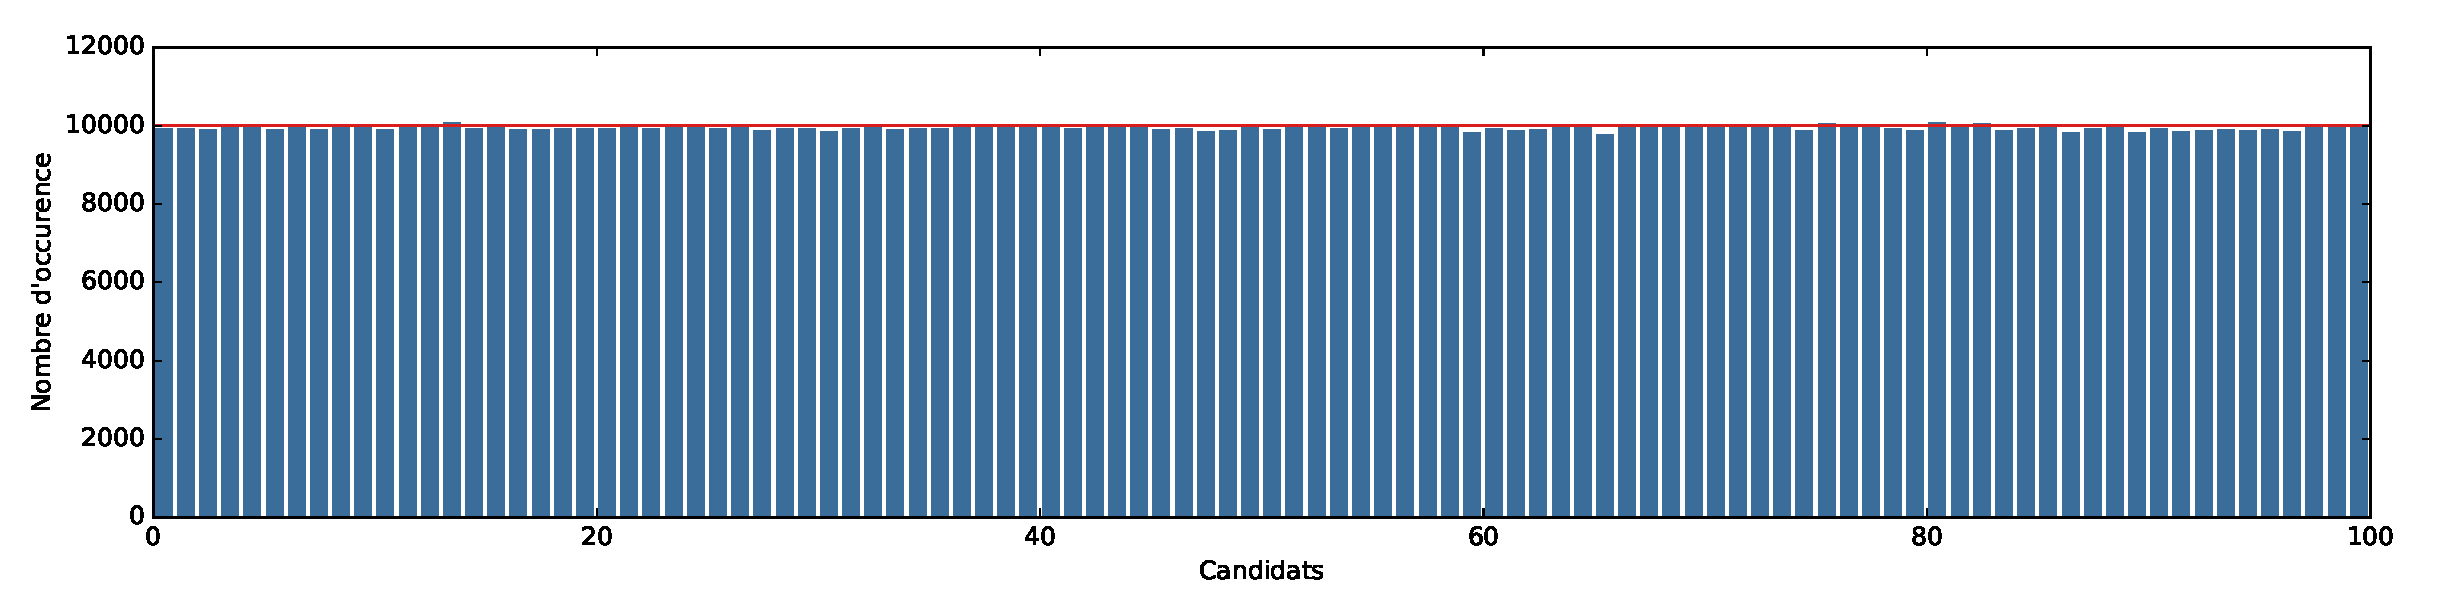
\includegraphics[width=0.98\textwidth]{../\rootPath image/lot_Nc-100_Ne-100000_Nl-10.pdf}
  \caption{Avec 100000 \'electeurs et 100 candidats, chaque candidat apparait autant de fois que les autres candidats dans les lots}
  \label{fig:scaling}
\end{figure*}

\begin{figure}[!ht]
  \centering
  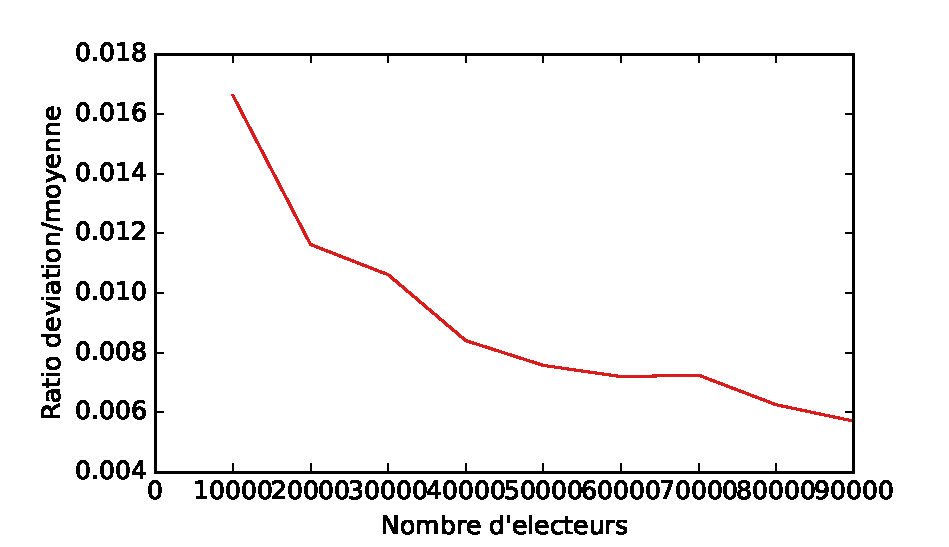
\includegraphics[width=0.98\columnwidth]{../\rootPath image/rsm_Nc-100_Nl-10.pdf}
  \caption{A partir de 30000 \'electeurs, le rapport \'ecart-type sur moyenne devient inf\'erieur \'a $1\%$.}
  \label{fig:scaling}
\end{figure}

\subsection{Nombre minimum d'\'electeurs}
\end{document}


